\documentclass{beamer}
\usepackage[utf8]{inputenc}
\usepackage[T1]{fontenc}
\usepackage{amsmath, amssymb}
\usepackage{graphicx}

% Paquetes para gráficas
\usepackage{pgfplots}
\pgfplotsset{compat=1.17}
\usetikzlibrary{positioning}

% Tema de la presentación
\usetheme{Madrid}

% Título, autor, etc.
\title{Métodos Numéricos de Interpolación}
\author{Claudio Cuevas Pazos}
\date{\today}

\begin{document}
	
	\frame{\titlepage}
	
	\begin{frame}
		\frametitle{Interpolación Lineal}
		La interpolación lineal consiste en aproximar una función mediante segmentos de recta entre los puntos dados. Dados dos puntos $(x_0, y_0)$ y $(x_1, y_1)$, la ecuación de la recta que pasa por ellos es:
		\[ y = y_0 + \frac{y_1 - y_0}{x_1 - x_0}(x - x_0) \]
		
		\begin{figure}
			\centering
			\begin{tikzpicture}
				\begin{axis}[
					width=0.7\textwidth,
					height=5cm,
					axis lines=middle,
					xlabel={$x$},
					ylabel={$y$},
					xmin=0, xmax=6,
					ymin=0, ymax=10,
					xtick={1, 4},
					ytick={2, 8},
					xticklabels={$x_0$, $x_1$},
					yticklabels={$y_0$, $y_1$},
					title={Interpolación Lineal}
					]
					\addplot[blue, domain=0:5, samples=100] {2 + (8 - 2) / (4 - 1) * (x - 1)};
					\addplot[red, only marks, mark=*] coordinates {(1, 2) (4, 8)};
				\end{axis}
			\end{tikzpicture}
		\end{figure}
	\end{frame}
	
	\begin{frame}
		\frametitle{Interpolación Log-Lineal}
		La interpolación log-lineal se utiliza para interpolar en el caso de datos positivos que varían exponencialmente. Consiste en interpolar en escala logarítmica y luego volver a la escala original. Dados dos puntos $(x_0, y_0)$ y $(x_1, y_1)$, la interpolación log-lineal se realiza como:
		\[ y = y_0 \left(\frac{y_1}{y_0}\right)^{\frac{x - x_0}{x_1 - x_0}} \]
		
		\begin{figure}
			\centering
			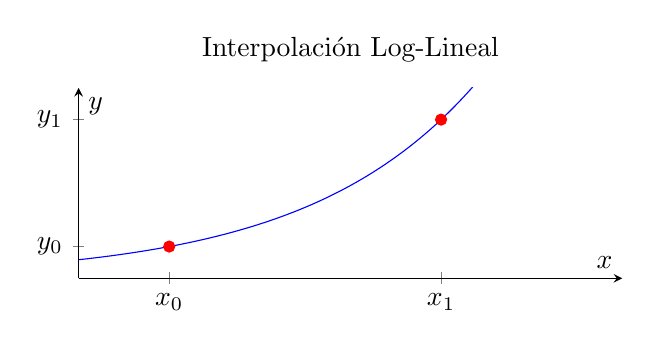
\begin{tikzpicture}
				\begin{axis}[
					width=0.7\textwidth,
					height=4cm,
					axis lines=middle,
					xlabel={$x$},
					ylabel={$y$},
					xmin=0, xmax=6,
					ymin=0, ymax=30,
					xtick={1, 4},
					ytick={5, 25},
					xticklabels={$x_0$, $x_1$},
					yticklabels={$y_0$, $y_1$},
					title={Interpolación Log-Lineal}
					]
					\addplot[blue, domain=0:5, samples=100] {5 * (25 / 5)^((x - 1) / (4 - 1))};
					\addplot[red, only marks, mark=*] coordinates {(1, 5) (4, 25)};
				\end{axis}
			\end{tikzpicture}
		\end{figure}
	\end{frame}
	
\begin{frame}
	\frametitle{Introducción a Splines Cúbicos}
	Los splines cúbicos son una técnica de interpolación que utiliza polinomios cúbicos para suavizar y conectar puntos de datos. La idea central detrás de los splines cúbicos es dividir el dominio en segmentos y usar polinomios cúbicos diferentes en cada segmento. Esto permite lograr una interpolación suave y diferenciable en los puntos de unión.
	
	\begin{itemize}
		\item Los splines cúbicos son funciones polinómicas de tercer grado.
		\item Los segmentos se definen por puntos de control.
		\item Se establecen condiciones de continuidad para garantizar suavidad.
	\end{itemize}
\end{frame}

\begin{frame}
	\frametitle{Definición Matemática}
	Dado un conjunto de puntos $(x_i, y_i)$, el spline cúbico $S_i(x)$ en el segmento $[x_i, x_{i+1}]$ se define como:
	\begin{align*}
		S_i(x) &= a_i + b_i (x - x_i) + c_i (x - x_i)^2 + d_i (x - x_i)^3
	\end{align*}
	
	Las incógnitas $a_i, b_i, c_i,$ y $d_i$ se determinan imponiendo condiciones en los puntos de unión y asegurando continuidad en la primera y segunda derivada.
\end{frame}

\begin{frame}
	\frametitle{Condiciones de Continuidad}
	Para garantizar suavidad y continuidad en los puntos de unión $x_i$:
	
	\begin{itemize}
		\item Continuidad en la función: $S_i(x_i) = y_i$ (interpolación).
		\item Continuidad en la primera derivada: $S_i'(x_i) = S_{i+1}'(x_i)$.
		\item Continuidad en la segunda derivada: $S_i''(x_i) = S_{i+1}''(x_i)$.
	\end{itemize}
	
	Estas condiciones generan un sistema de ecuaciones lineales que se resuelve para obtener los coeficientes del spline cúbico en cada segmento.
\end{frame}

\begin{frame}
	\frametitle{Ejemplo Numérico}
	Supongamos que tenemos los puntos $(x_0, y_0)$, $(x_1, y_1)$, $(x_2, y_2)$, y $(x_3, y_3)$, y deseamos construir un spline cúbico para interpolar entre ellos.
	
	\begin{align*}
		S_0(x) &= a_0 + b_0 (x - x_0) + c_0 (x - x_0)^2 + d_0 (x - x_0)^3 \\
		S_1(x) &= a_1 + b_1 (x - x_1) + c_1 (x - x_1)^2 + d_1 (x - x_1)^3 \\
		S_2(x) &= a_2 + b_2 (x - x_2) + c_2 (x - x_2)^2 + d_2 (x - x_2)^3 \\
		S_3(x) &= a_3 + b_3 (x - x_3) + c_3 (x - x_3)^2 + d_3 (x - x_3)^3
	\end{align*}
	
	Los coeficientes se determinan resolviendo el sistema de ecuaciones resultante de aplicar las condiciones de continuidad y los valores en los puntos de datos.
\end{frame}

\begin{frame}
	\frametitle{Ejemplo de Spline Cúbico}
	\begin{figure}
		\centering
		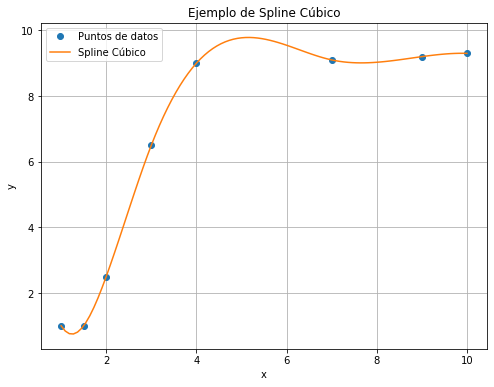
\includegraphics[width=0.7\textwidth]{spline_example.png}
		\caption{Ejemplo de Spline Cúbico}
	\end{figure}
\end{frame}

\begin{frame}
	\frametitle{Resolución de Sistemas Tridiagonales}
	El cálculo de los coeficientes de los splines cúbicos involucra la resolución de un sistema de ecuaciones tridiagonal. Este sistema es generado por las condiciones de continuidad y suavidad impuestas en los splines cúbicos.
	
	\begin{itemize}
		\item Los coeficientes de los splines cúbicos se calculan en cada segmento.
		\item Se utiliza un algoritmo de eliminación gaussiana modificado.
		\item El sistema tridiagonal se resuelve en función de las segundas derivadas de los splines.
	\end{itemize}
\end{frame}

\begin{frame}
	\frametitle{Sistema Tridiagonal}
	Supongamos que tenemos $n+1$ puntos de datos $(x_0, y_0), (x_1, y_1), \ldots, (x_n, y_n)$ y queremos calcular los coeficientes de los splines cúbicos para interpolar entre ellos.
	
	El sistema tridiagonal tiene la forma:
	
	\[
	\begin{bmatrix}
		B_1 & C_1 & 0 & 0 & \ldots & 0 \\
		A_2 & B_2 & C_2 & 0 & \ldots & 0 \\
		0 & A_3 & B_3 & C_3 & \ldots & 0 \\
		\vdots & \vdots & \vdots & \vdots & \ddots & \vdots \\
		0 & 0 & \ldots & 0 & A_n & B_n
	\end{bmatrix}
	\begin{bmatrix}
		m_0 \\
		m_1 \\
		m_2 \\
		\vdots \\
		m_n
	\end{bmatrix}
	=
	\begin{bmatrix}
		d_1 \\
		d_2 \\
		d_3 \\
		\vdots \\
		d_n
	\end{bmatrix}
	\]
	
	Donde $A_i$, $B_i$, y $C_i$ son coeficientes, y $d_i$ se calculan a partir de las diferencias entre puntos.
\end{frame}

\begin{frame}
	\frametitle{Algoritmo de Eliminación Gaussiana Modificado}
	La eliminación gaussiana modifiada es utilizada para resolver el sistema tridiagonal. El algoritmo consiste en tres pasos principales:
	
	\begin{enumerate}
		\item Eliminación hacia adelante: Se descompone la matriz en una matriz triangular superior.
		\item Sustitución hacia atrás: Se calculan las soluciones para el sistema.
		\item Cálculo de coeficientes: Se obtienen los coeficientes del spline cúbico en cada segmento.
	\end{enumerate}
	
	Este algoritmo permite obtener las segundas derivadas $m_i$ de los splines cúbicos, lo que a su vez nos da los coeficientes necesarios para definir los splines cúbicos en cada segmento.
\end{frame}

\begin{frame}
	\frametitle{Ejemplo Numérico}
	Supongamos que tenemos los puntos $(x_0, y_0)$, $(x_1, y_1)$, $(x_2, y_2)$ y $(x_3, y_3)$ y queremos calcular los coeficientes de los splines cúbicos para interpolar entre ellos.
	
	\begin{align*}
		&h_1 = x_1 - x_0, \quad h_2 = x_2 - x_1, \quad h_3 = x_3 - x_2 \\
		&\text{Calculamos } \alpha_i = \frac{3}{h_i}(a_{i+1} - a_i) - \frac{3}{h_{i-1}}(a_i - a_{i-1}) \\
		&\text{Formamos las matrices tridiagonales:} \\
		&A = \begin{bmatrix}
			h_1 & 2(h_1 + h_2) & h_2 & 0 \\
			0 & h_2 & 2(h_2 + h_3) & h_3 \\
			& & \ddots & \ddots & \ddots \\
		\end{bmatrix} \\
		&\mathbf{m} = \begin{bmatrix}
			m_1 \\
			m_2 \\
			\vdots
		\end{bmatrix}, \quad \mathbf{d} = \begin{bmatrix}
			\alpha_1 \\
			\alpha_2 \\
			\vdots
		\end{bmatrix}
	\end{align*}
\end{frame}

\begin{frame}
		Resolvemos el sistema tridiagonal $A \mathbf{m} = \mathbf{d}$ utilizando el algoritmo de eliminación gaussiana modificado y luego calculamos los coeficientes del spline cúbico en cada segmento.
\end{frame}
	
\end{document}
